\section{Theory}
\label{sec:theory}

\subsection{Photoluminescence}

To probe the band gap of semiconductors, photoluminescence spectroscopy can be used.
This means illuminating the sample in order to create electron-hole pairs, which then form excitons and ultimately recombine.
The energy of the exciton annihilation is characteristic for the material.
Therefore a spectrum recorded by the emission of such an illuminated sample will contain a peak at this characteristic energy (wavelength) as well as possibly other peaks stemming from effects such as spin-splitting and phonon-activated transitions.

\subsection{Transition metal dichalcogenides}

Transition metal dichalcogenides (TMDCs) are layered materials made from one part transition metal (Mo, Ti, W) and two parts chalcogenides (S, Se, Te) and are typically semiconductors.
The general crystal structure is shown in \cref{fig_tmdc_structure}.
The layers can be separated from each other by exfoliation as they are only bound by comparatively weak Van der Waals bonds, while within the plane the atoms are bound by covalent bonds.
As monolayers unlike the bulk crystal don't have an inversion center, the band structure changes considerably, when moving to monolayers from the bulk.
Specifically the $\hbar{K}$ points of the reciprocal lattice no longer show sixfold symmetry, and split into $\hbar{K}$ and $\hbar{K}'$, which have reversed splin splitting.
As shown in \cref{fig_valley_split}, this leads to the existence of lower energy A excitons and higher energy B excitons.

\begin{figure}[!ht]
    \centering
    \begin{subfigure}{0.47\textwidth}
        \centering
    		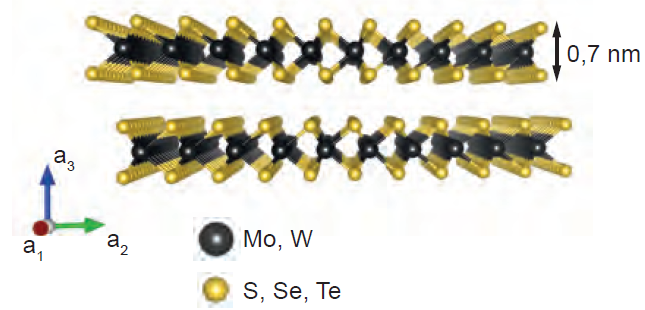
\includegraphics[width=\textwidth]{img/tmdc_structure.png}
    		\caption{} %TODO schauen, ob das auch mit doctorsthesis funktioniert,
    		\label{fig_tmdc_structure}
    \end{subfigure}
    \hfill
    \begin{subfigure}{0.37\textwidth}
        \centering
        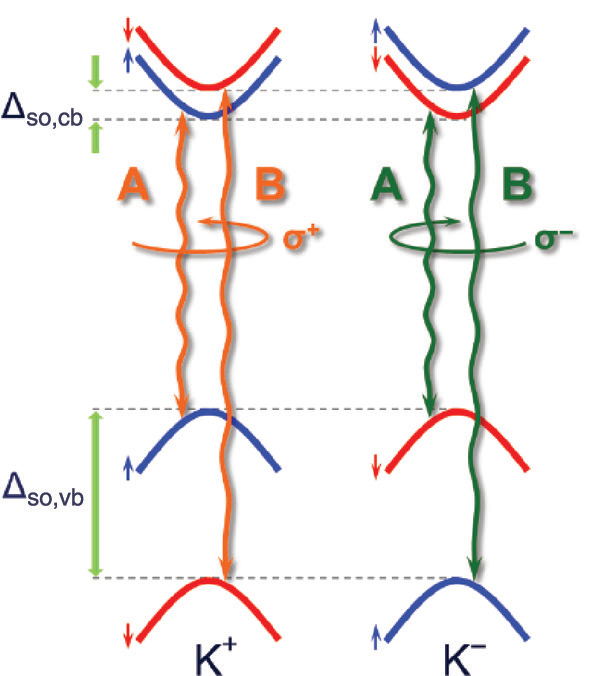
\includegraphics[width=\textwidth]{img/AB_exc.png}
        \caption{}
	      \label{fig_valley_split}
    \end{subfigure}
    \caption{a: Layered crystal structure of TMDCs. \cite{Schmidt2016}. b: Valley dependence on spin splitting in monolayer TMDCs.\cite{Koperski2017} }
	\label{fig_tmdcs} % 3->1
\end{figure}


\subsection{Single-photon emitters}
\label{sec:theory:spe}

Single-photon emitters (SPEs) are light sources that don't emit more than one photon at once.
SPEs are identified, by performing photon antibunching, meaning that two detectors are used whith one giving a start signal and the other the stop signal, allowing the measurement of the second-order correlation function $g^{(2)}(\tau)$.
If the emitter in question is a Single-photon emitter, there will be a significant dip in the relative quantity of delays between start and stop signal close to zero.

\subsection{Magneto-optic effect}

	The interaction of electromagnetic waves with matter can be described with the refractive index
	\begin{align*}
		\tilde{n} = n + ik \,,
	\end{align*}
	where $n$ describes the refraction and $k$ the absorption.
	From this, information on reflection and transmission can also be extracted.
	Adding an external magnetic field to the matter, changes its refractive index for different polarizations of the incoming electromagnetic wave.
	Linear polarized light can be described by a superposition of two circular polarized electromagnetic waves, one left- and one right-polarized.
	When passing through the matter, the left- and right-polarized parts of linear polarized light change differently in intensity and phase.
	The result is that the superposition of both waves no longer adds to linear polarized, but elliptic polarized light.
	From the phase change results a rotation of the lights main oscillation axis and from the intensity change the ellipticity.
	This rotation is also known as faraday rotation.
	Here, it should be noted that this is for the transmission through matter, on the other hand for reflection a similiar effect, namely the magneto-optical kerr effect, takes place.

	\

	As the change in polarizations through interaction with magnetized matter is heavily dependent on the properties of the matter, band structure information can be obtained using magneto-optic methods.
	An example for this is given by spin polarized band gaps.
	For this investigation, the Zeeman-splitting for 1s-excitons in TMDCs and how they influence the refractive properties of matter is of interest.
	This can be described by the verdet constant which is given by:
	\begin{align*}
		V = \frac{\varphi_\text{F}}{L\cdot B} \,,
	\end{align*}
	where $\varphi_\text{F}$ is the faraday rotation, $L$ the thickness of the sample and $B$ the magnetic field strength of the external field.

	To allow the deduction of the faraday rotation by measurement of transmission intensities, Jones matrices can be used.
	They describe the change of polarisation in the plane transverse to the light's direction of propagation.
	For example the sample can be described by
	\begin{align*}
		\hat{\text{S}} = \left( \begin{array}{rr}
		1 & (\varphi_\text{F} + i\eta_\text{F}) \\
		-(\varphi_\text{F} + i\eta_\text{F}) & 1 \\
	\end{array}\right) \,.
	\end{align*}
	The initial linear polarized light $\hat{E}_i$ can be written as a two-component vector:
	\begin{align*}
		\hat{E}_i = \left( \begin{array}{r}
					\cos{p} \\
					\sin{p} \\
				\end{array}\right) \,,
	\end{align*}
	$p$ being the polarisation.
	By multiplying this vector with the Jones matrices of the different objects in the beams path, expressions for the measured intensities $T_i = E_i* E_i$ can be calculated.
  Specifically, $E_i \propto \text{Jones matrices} \cdot \hat{E}_i$.
  The faraday rotation results from taking the difference of the measured intensities $T_i$ each divided by the intensities measured without a sample $T_i^0$:
	\begin{align*}
		\frac{T_1}{T_1^0} - \frac{T_2}{T_2^0} = 4 \varphi_\text{F} + \varphi_\text{bg} \,.
	\end{align*}
	Here, the indexes $1$ and $2$ are assigned to the two components of the initially linear polarized light.
	Additionally, there is $\varphi_\text{bg}$ which amounts to noise which is also expected to be measured.
